\subsection{Overview}
The basic architecture for the system is a Client-Server setup. The server will handle persistent data and contain a small subsystem for manipulating data, we will for now not describe the server or the communication between the server and client greater detail and instead focus on the client.\\

The Client-system will be made with a Model-View-Controller (MVC) architecture. The system should have different views (Log in, MonthView... etc.) which would require different event-handling. The MVC allows this because it makes it easy to do runtime changes of views and controllers. It also results in high cohesion, in that the control objects and the view objects are separated in accordance to their respective responsibilities. Both view and control objects can be separated into small classes that only handles smaller tasks. However creating the MVC-architecture requires extra code. The main architecture can be seen below (it is possible to zoom in), we have not included all views and control objects to keep things a bit clean.

\paragraph{Architecture}
\begin{center}
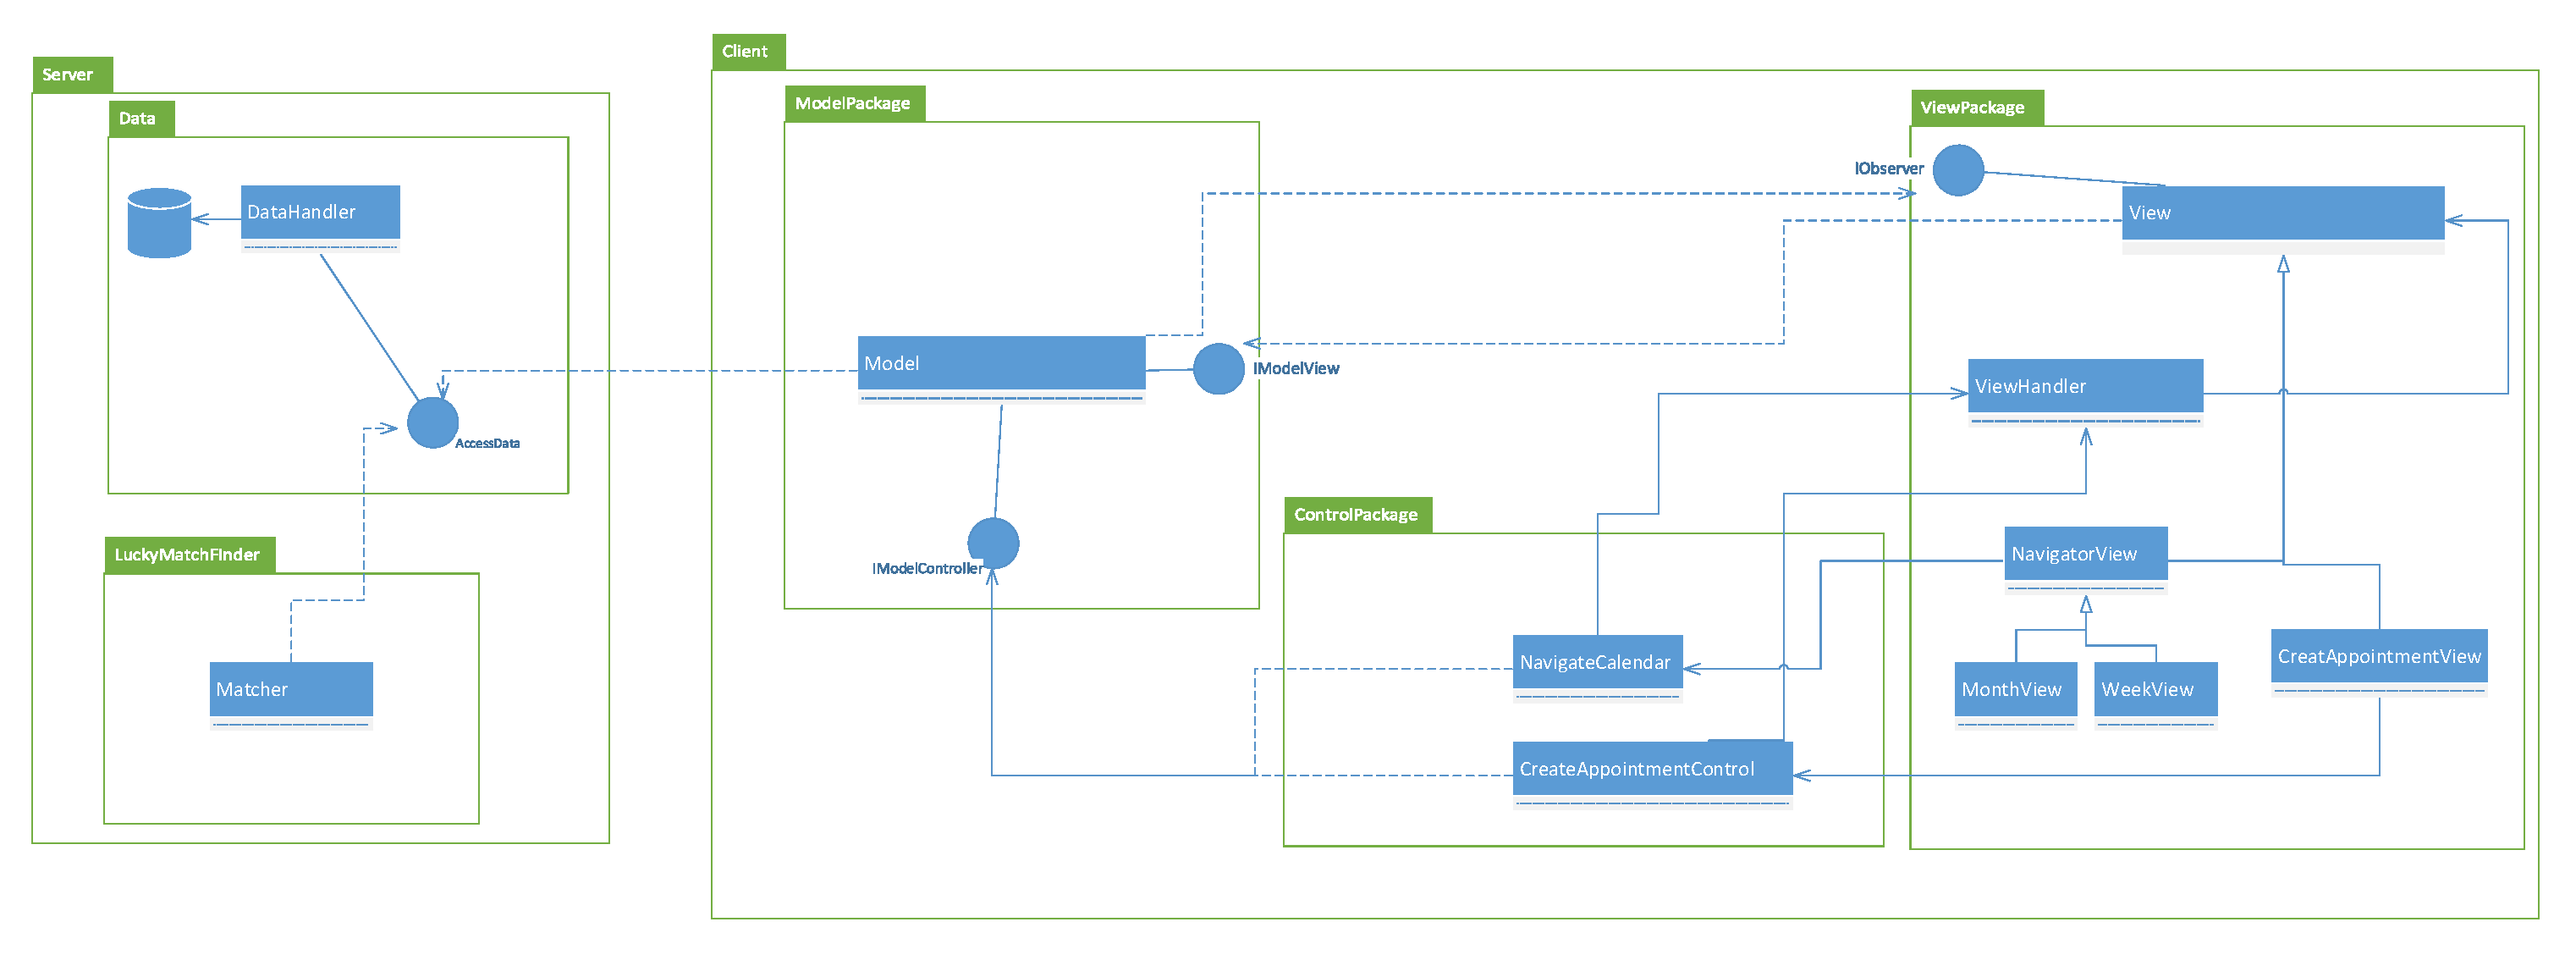
\includegraphics[scale=.4]{sections/Architecture.pdf}
\end{center}
\pagebreak

\subsection{Subsystem decomposition}
The MVC architecture gives us three distinct types of subsystems, a model that handles date, a view that handles UI, and a Control object that handles event-flow and manipulation of data. The model subsystem should function independently from the rest of the system, therefore we used a facade design pattern to hide the internal implementation of the model from the rest of the system. In addition, the model communicates with the different views through a Observer/Observable-pattern, which mean the model isn't coupled to the Views.\\

The rest of the system is divided into View and Control objects. Each View requires a Control object, that handles the event-flow of the View. Each Control object has a reference to the ViewHandler, which allows them to create a new View when necessary. \\

At this point we have identified three types of views, a NavigatorView that shows calendar navigation, a AppointmentView that shows an appointment, and a login view that allows a guest to log-in and/or create a user. Each view have one of several control objects, which handles the events caused by the user. There might be several View objects for each Control object fx. the NavigateCalender control object could be responsible for MonthView, WeekView, and DayView under the common name NavigatorView. However, the opposite is not true. One view object cannot be controlled by more than one control object. 

\subsection{Hardware/software mapping}
Since our system uses the Client-Server pattern, we need an independent server, that stores all data centrally and runs our LuckyMatchFinder algorithm. The server communicates through a http-connection with a user logged on locally through the client subsystem. The connection is handled by the DataHandler subsystem on the server and the Model subsystem on the Client. The DataHandler part on the server encapsulates a SQL-database. The Client is also able to save data locally, if unable to connect to the server. The Model uses a Bridge pattern to apply the different data handling interfaces, these are assigned through an Abstract factory.


\subsection{Persistent data management}
We have identified the following persistent objects; APPOINTMENTS, LUCKYAPPOINTMENTS, USERS and NOFICATIONS. They are all saved by the server subsystem in a relational Database. When the user logs in, the Client synchronizes the users APPOINTMENTS, LUCKYAPPOINTMENTS and NOTIFICATIONS with the server, so that the Client subsystem is up to date with the changes, and the system can be used without connection. If local changes have not been saved to the server (probably due to loss of network connection), the system will synchronize next time a connection is established. This also means, that if a user has logged in to the system on a machine, it is possible to log in without connection later on, since the user-data is stored locally. There might be some problems with security or long periods without login, so we have yet to decide finer details of the synchronization between the Client and Server.

We considered saving persistent boundary objects locally, such as user preferences and last shown view, but we decided against it, since the client is supposed to be simple and intuitive, with ease of use and accessibility as declared design goals, making these boundary objects persistent, should not be necessary. 


\subsection{Access control and security}
In our system all users have the same access to the all actions related to their appointment. Users are defined as authenticated users, so the user has already been through the authentication process and can only access its own appointments. All users that have been added normally to an appointment are participants and all have access to edit the appointment. The users added to the the appointment to the LuckyMatchFinder by making a LuckyAppointment are defined as LuckyParticipants and do not have any possibilities to edit the Appointment.\\

We will not encrypt the data transfer of the appointments to between the server and the client, but we wish to encrypt the transfer of the user names by with the password as the key, so that only the user is allowed to his own username and the server then stores the usernames and links them to the relevant appointments, so the authenticated user can access them. \\

No one is allowed to delete an appointment, an appointment is deleted when the last participants leaves. 
However a participant may remove other participants from an appointment, which in reality gives the power of delete appointment.

{\tabulinesep=1.2mm
\begin{tabu}{ | p{3cm} | p{6cm} | p{6cm} |}
    \hline
     	 			        & 		Participant         &		LuckyParticipant \\ \hline
    EditAppointment         &       +					&		-          \\\hline
    LeaveAppointment        &       +					&		+      \\ \hline
    RemoveParticipants		&		+					&		- 		\\\hline
    DeleteAppointment       &       -					&		-        \\  \hline
\end{tabu}
}

+ access matrix??
 
\subsection{Global software control}
The Client will generally be using an event-driven control flow. There will be a main-loop listening to for GUI-events and when an event happens it is handled by the relevant controller-class. We still might want to have several threads running, e.g. the ConnectionHandler. Similarly the AppointmentMatcher running on the server will probably be pretty procedural as it is run x times a day and never even waits events.



\subsection{Boundary conditions}
We have identified the following boundary conditions on the client and the server:


\begin{itemize}
	\item Configuration:
	\begin{enumerate}
		\item We have found no undefined changes to persistent data in our use cases. All changes to appointments has been accounted for by either the user or the server
	\end{enumerate}
	\Item Start-up and Shutdown:
	\begin{enumerate}
		\item We had no use cases which included Start-up or shutdown for either the client or the server. We have added the ServerAdmin actor in our use cases and given him the use case ManageServer which includes starting and shutting down the server. We found it to trivial to describe in greater detail.
		\item With regards to the clients startup and shutdown, we found it too trivial to make real use cases for it. They are already specified in the Users use cases as entry and exit conditions
	\end{enumerate}
	\Item Exception handling:
	\begin{enumerate}
		\item We have identified the scenario where the client looses connection to the server as the biggest threat in our system. We therefore added functionality for the client to save data locally after loosing connection with the server and synchronize the data when the connection is reestablished. (Operating environment)
		\item We realize that both the Client and the Server is open for hardware-failures, but we have chosen to address this at a later point, when we know more about the specific hardware that this software will run on (Hardware-failures)
	\end{enumerate}
\end{itemize}
